\documentclass{article}

\usepackage[spanish]{babel}
\setlength{\parskip}{\medskipamount}
\setlength{\parindent}{0pt}
\usepackage[utf8]{inputenc}
\DeclareUnicodeCharacter{00B5}{\ensuremath{\mu}}
\usepackage{graphicx}
\usepackage{color}
\usepackage{amsmath}
\usepackage{ifthen}
\usepackage{amssymb}
\usepackage{float}
\usepackage{amsmath}
\newsavebox{\picturebox}
\newlength{\pictureboxwidth}
\newlength{\pictureboxheight}
\newcommand{\includeimage}[1]{
    \savebox{\picturebox}{\includegraphics{#1}}
    \settoheight{\pictureboxheight}{\usebox{\picturebox}}
    \settowidth{\pictureboxwidth}{\usebox{\picturebox}}
    \ifthenelse{\lengthtest{\pictureboxwidth > .95\linewidth}}
    {
        \includegraphics[width=.95\linewidth,height=.80\textheight,keepaspectratio]{#1}
    }
    {
        \ifthenelse{\lengthtest{\pictureboxheight>.80\textheight}}
        {
            \includegraphics[width=.95\linewidth,height=.80\textheight,keepaspectratio]{#1}
            
        }
        {
            \includegraphics{#1}
        }
    }
}
\DeclareMathOperator{\abs}{abs}
\usepackage{animate} % This package is required because the wxMaxima configuration option
                      % "Export animations to TeX" was enabled when this file was generated.

\definecolor{labelcolor}{RGB}{100,0,0}

\begin{document}
%%%%%%%%%%%%%%%%%%%%%%%%%%

%	EJEMPLOS

%%%%%%%%%%%%%%%%%%%%%%%%%%
{\Huge {\sc Ejemplo}}\\

Polinomio de grado 5:\quad $f(x)=2x^5+6x^4+2x^2-6x$

La sucesión de Sturm es:

$$f_0(x) = 2\cdot {{x}^{5}}+6\cdot {{x}^{4}}+2\cdot {{x}^{2}}-6\cdot x$$\\
$$f_1(x) = 10\cdot {{x}^{4}}+24\cdot {{x}^{3}}+4\cdot x-6$$\\
$$f_2(x) = \frac{-18+132\cdot x-30\cdot {{x}^{2}}+72\cdot {{x}^{3}}}{25}$$\\
$$f_3(x) = \frac{-75+3250\cdot x+475\cdot {{x}^{2}}}{72}$$\\
$$f_4(x) = -\frac{1342656\cdot x-36288}{9025}$$\\
$$f_5(x) = -\frac{9025}{49284}$$\\
\\
Las raíces estarán en el intervalo [-4,4].

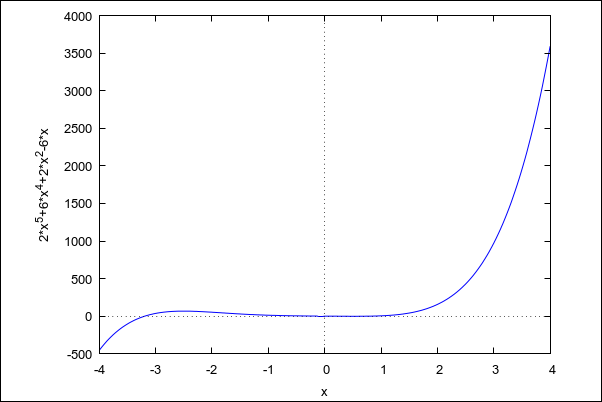
\includegraphics[scale=0.5]{img/1}


\begin{table}[h]
\centering
\label{my-label}
\begin{tabular}{|l|l|l|}
\hline
                            & -4 & 4 \\ \hline
Número de  cambios de signo & 4  & 1 \\ \hline
\end{tabular}
\end{table}

\begin{table}[h]
\centering
\label{my-label}
\begin{tabular}{|l|l|l|l|}
\hline
                            & -4 & 0 & 4 \\ \hline
Número de  cambios de signo & 4  & 2 & 1 \\ \hline
\end{tabular}
\end{table}

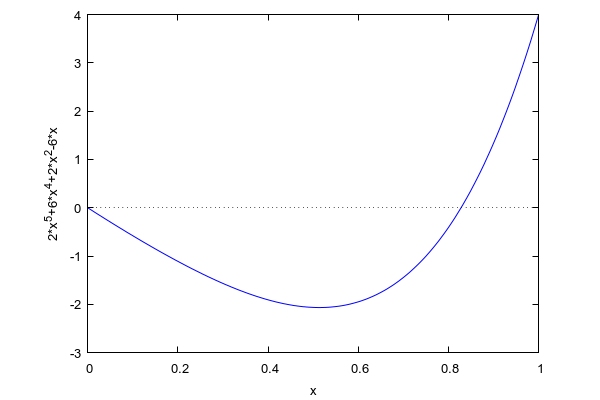
\includegraphics[scale=0.4]{img/2}

\begin{table}[h]
\centering
\label{my-label}
\begin{tabular}{|l|l|l|l|}
\hline
                            & -4 & -2 & 0 \\ \hline
Número de  cambios de signo & 4  & 3  & 2 \\ \hline
\end{tabular}
\end{table}

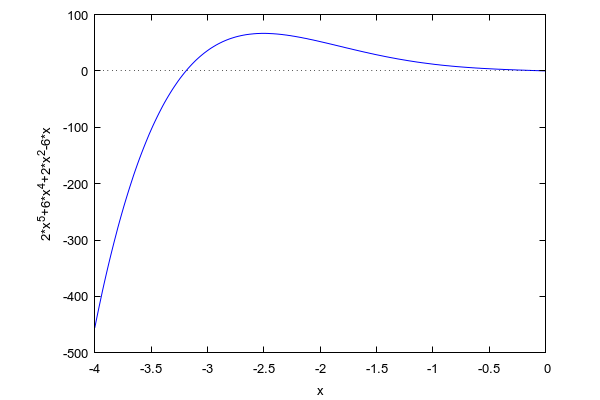
\includegraphics[scale=0.4]{img/3}

\newpage

%%%%%%%%%%%%%%%%%%%%%%%%%%

%	EJERCICIO 10

%%%%%%%%%%%%%%%%%%%%%%%%%%
{\Huge {\sc Ejercicio 10}}\\

Considera la función $g(x) = \lambda x(1 - x)$, con $\lambda \in [0, 4]$.\\

a) Demuestra que $g([0, 1]) \subset [0, 1]$.\\

b) Calcula los puntos fijos de la función en [0, 1] en función de $\lambda$.\\

c) Considera la sucesión de iteraciones $x_{n+1} = g(x_n), n = 0, 1,\dots$ y analiza la convergencia de dicha sucesión a los puntos fijos de $g$, en función de $\lambda$.\\

%%%%%%%%%%%%%%%%%%%%%%%%%%

%	EJERCICIO 14

%%%%%%%%%%%%%%%%%%%%%%%%%%
{\Huge {\sc Ejercicio 14}}\\

Considera el polinomio $p(x) = 2x^5 - x^4 - 4x^3 + 2x^2 - 6x + 3$.\\
a) Calcula una sucesión de Sturm asociada a $p(x)$.\\

$$f_0(x) = 2\cdot {{x}^{5}}-{{x}^{4}}+4\cdot {{x}^{3}}+2\cdot {{x}^{2}}-6\cdot x+3$$\\
$$f_1(x) = 10\cdot {{x}^{4}}-4\cdot {{x}^{3}}+12\cdot {{x}^{2}}+4\cdot x-6$$\\
$$f_2(x) = -\frac{72-118\cdot x+36\cdot {{x}^{2}}+38\cdot {{x}^{3}}}{25}$$\\
$$f_3(x) = -\frac{7050-20500\cdot x+20150\cdot {{x}^{2}}}{361}$$\\
$$f_4(x) = -\frac{8987456\cdot x-7451040}{4060225}$$\\
$$f_5(x) = \frac{1181525475}{109253762}$$\\
\\

b) Halla una cota superior e inferior de las raíces de $p(x)$.\\

c) Localiza todas las raíces reales de $p(x)$ en un intervalo cada una.\\

\begin{table}[h]
\centering
\label{my-label}
\begin{tabular}{|l|l|l|}
\hline
                            & -4 & 4 \\ \hline
Número de  cambios de signo & 4  & 1 \\ \hline
\end{tabular}
\end{table}

\begin{table}[h]
\centering
\label{my-label}
\begin{tabular}{|l|l|l|l|}
\hline
                            & -4 & 0 & 4 \\ \hline
Número de  cambios de signo & 4  & 3 & 1 \\ \hline
\end{tabular}
\end{table}

\begin{table}[h]
\centering
\label{my-label}
\begin{tabular}{|l|l|l|l|}
\hline
                            & 0 & 2 & 4 \\ \hline
Número de  cambios de signo & 3 & 1 & 1 \\ \hline
\end{tabular}
\end{table}

\begin{table}[H]
\centering
\label{my-label}
\begin{tabular}{|l|l|l|l|}
\hline
                            & 0 & 1 & 2 \\ \hline
Número de  cambios de signo & 3 & 2 & 1 \\ \hline
\end{tabular}
\end{table}


%%%%%%%%%%%%%%%%%%%%%%%%%%

%	EJERCICIO 18

%%%%%%%%%%%%%%%%%%%%%%%%%%
{\Huge {\sc Ejercicio 18}}\\

Considera el sistema de ecuaciones:
$$g(x) = \left\{
\begin{array}{c l}
 3x_1 - cos(x_2x_3) - \frac{1}{2}        &= 0\\
 x_1^2 - 81(x_2+0.1)^2 + sin(x_3) + 1.06 &= 0\\
 e^{-x_1x_2} + 20x_3 + \frac{10\pi-3}{3} &= 0
\end{array}
\right.
$$

a) Escribe el sistema anterior en la forma $x = g(x)$ despejando en la ecuación $i$ la variable $x_i$ , $i = 1, 2, 3$.

$$g(x) = \begin{pmatrix}
    x_1 \\
    x_2 \\
    x_3     
\end{pmatrix}
=\begin{pmatrix}
    \frac{cos(x_2x_3)+\frac{1}{2}}{3} \\
    \sqrt{\frac{sin(x_3)+x_1^2+1.06}{81}}-0.1 \\
    \frac{e^{-x_1x_2}+ \frac{10\pi-3}{3}}{-20}     
\end{pmatrix}$$

b) Demuestra, utilizando el resultado del ejercicio anterior que el sistema de ecuaciones tiene una única solución en
$$D = \{(x_1 , x_2 , x_3) \in \mathbb{R}^3 | 1 \le x_i \le 1, i = 1, 2, 3\}$$

\noindent
%%%%%%%%%%%%%%%
%%% INPUT:
\begin{minipage}[t]{8ex}\color{red}\bf
\begin{verbatim}
-->  
\end{verbatim}
\end{minipage}
\begin{minipage}[t]{\textwidth}\color{blue}
\begin{verbatim}
diff(g1(x,y,z),x);
\end{verbatim}
\end{minipage}
%%% OUTPUT:

\[\displaystyle
\parbox{10ex}{$\color{labelcolor}\mathrm{\tt (\%o33) }\quad $}
0\mbox{}
\]
%%%%%%%%%%%%%%%


\noindent
%%%%%%%%%%%%%%%
%%% INPUT:
\begin{minipage}[t]{8ex}\color{red}\bf
\begin{verbatim}
-->  
\end{verbatim}
\end{minipage}
\begin{minipage}[t]{\textwidth}\color{blue}
\begin{verbatim}
diff(g1(x,y,z),y);
\end{verbatim}
\end{minipage}
%%% OUTPUT:

\[\displaystyle
\parbox{10ex}{$\color{labelcolor}\mathrm{\tt (\%o34) }\quad $}
-\frac{z\cdot \mathrm{sin}\left( y\cdot z\right) }{3}\mbox{}
\]
%%%%%%%%%%%%%%%


\noindent
%%%%%%%%%%%%%%%
%%% INPUT:
\begin{minipage}[t]{8ex}\color{red}\bf
\begin{verbatim}
-->  
\end{verbatim}
\end{minipage}
\begin{minipage}[t]{\textwidth}\color{blue}
\begin{verbatim}
diff(g1(x,y,z),z);
\end{verbatim}
\end{minipage}
%%% OUTPUT:

\[\displaystyle
\parbox{10ex}{$\color{labelcolor}\mathrm{\tt (\%o35) }\quad $}
-\frac{y\cdot \mathrm{sin}\left( y\cdot z\right) }{3}\mbox{}
\]
%%%%%%%%%%%%%%%


\noindent
%%%%%%%%%%%%%%%
%%% INPUT:
\begin{minipage}[t]{8ex}\color{red}\bf
\begin{verbatim}
-->  
\end{verbatim}
\end{minipage}
\begin{minipage}[t]{\textwidth}\color{blue}
\begin{verbatim}
diff(g2(x,y,z),x);
\end{verbatim}
\end{minipage}
%%% OUTPUT:

\[\displaystyle
\parbox{10ex}{$\color{labelcolor}\mathrm{\tt (\%o36) }\quad $}
\frac{x}{9\cdot \sqrt{\mathrm{sin}\left( z\right) +{{x}^{2}}+1.06}}\mbox{}
\]
%%%%%%%%%%%%%%%


\noindent
%%%%%%%%%%%%%%%
%%% INPUT:
\begin{minipage}[t]{8ex}\color{red}\bf
\begin{verbatim}
-->  
\end{verbatim}
\end{minipage}
\begin{minipage}[t]{\textwidth}\color{blue}
\begin{verbatim}
diff(g2(x,y,z),y);
\end{verbatim}
\end{minipage}
%%% OUTPUT:

\[\displaystyle
\parbox{10ex}{$\color{labelcolor}\mathrm{\tt (\%o37) }\quad $}
0\mbox{}
\]
%%%%%%%%%%%%%%%


\noindent
%%%%%%%%%%%%%%%
%%% INPUT:
\begin{minipage}[t]{8ex}\color{red}\bf
\begin{verbatim}
-->  
\end{verbatim}
\end{minipage}
\begin{minipage}[t]{\textwidth}\color{blue}
\begin{verbatim}
diff(g2(x,y,z),z);
\end{verbatim}
\end{minipage}
%%% OUTPUT:

\[\displaystyle
\parbox{10ex}{$\color{labelcolor}\mathrm{\tt (\%o38) }\quad $}
\frac{\mathrm{cos}\left( z\right) }{18\cdot \sqrt{\mathrm{sin}\left( z\right) +{{x}^{2}}+1.06}}\mbox{}
\]
%%%%%%%%%%%%%%%


\noindent
%%%%%%%%%%%%%%%
%%% INPUT:
\begin{minipage}[t]{8ex}\color{red}\bf
\begin{verbatim}
-->  
\end{verbatim}
\end{minipage}
\begin{minipage}[t]{\textwidth}\color{blue}
\begin{verbatim}
diff(g3(x,y,z),x);
\end{verbatim}
\end{minipage}
%%% OUTPUT:

\[\displaystyle
\parbox{10ex}{$\color{labelcolor}\mathrm{\tt (\%o39) }\quad $}
\frac{\mathrm{log}\left( e\right) \cdot y}{20\cdot {{e}^{x\cdot y}}}\mbox{}
\]
%%%%%%%%%%%%%%%


\noindent
%%%%%%%%%%%%%%%
%%% INPUT:
\begin{minipage}[t]{8ex}\color{red}\bf
\begin{verbatim}
-->  
\end{verbatim}
\end{minipage}
\begin{minipage}[t]{\textwidth}\color{blue}
\begin{verbatim}
diff(g3(x,y,z),y);
\end{verbatim}
\end{minipage}
%%% OUTPUT:

\[\displaystyle
\parbox{10ex}{$\color{labelcolor}\mathrm{\tt (\%o40) }\quad $}
\frac{\mathrm{log}\left( e\right) \cdot x}{20\cdot {{e}^{x\cdot y}}}\mbox{}
\]
%%%%%%%%%%%%%%%

\noindent
%%%%%%%%%%%%%%%
%%% INPUT:
\begin{minipage}[t]{8ex}\color{red}\bf
\begin{verbatim}
-->  
\end{verbatim}
\end{minipage}
\begin{minipage}[t]{\textwidth}\color{blue}
\begin{verbatim}
diff(g3(x,y,z),z);
\end{verbatim}
\end{minipage}
%%% OUTPUT:

\[\displaystyle
\parbox{10ex}{$\color{labelcolor}\mathrm{\tt (\%o41) }\quad $}
0\mbox{}
\]
%%%%%%%%%%%%%%%

c) Calcula una aproximación de la solución con el método de iteración funcional
tomando $x^{(0)}$ = (0.1, 0.1, -0.1) con una tolerancia fijada de $10^{-5}$, donde la tolerancia viene dada por la norma infinito de la diferencia de dos aproximaciones sucesivas.

Todos las aproximaciones de la primera variante\\

Aproximación: (0.499983333472222, 0.00944114960371334, -0.523101267285757), punto: (0.499995934919313, 0.0000255677467667359, -0.523363310908805), distancia entre términos: 0.423101267285757\\

Aproximación: (0.499995934919313, 0.0000255677467667359, -0.523363310908805), punto: (0.499999999970157, 0.0000123367203633540, -0.523598136413912), distancia entre términos: 0.00941558185694660\\

Aproximación: (0.499999999970157, 0.0000123367203633540, -0.523598136413912), punto: (0.499999999993046, 3.41679062543232e-8, -0.523598467181241), distancia entre términos: 0.000234825505107006\\

Aproximación: (0.500000000000000, 1.64870403995820e-8, -0.523598774744101), punto: (0.500000000000000, 4.56640003587694e-11, -0.523598775186123), distancia entre términos: 3.07562860180077e-7

d) Sabiendo que la solución del sistema es $x^{*} = \left(0.5, 0, \frac{-\pi}{6}\right)$ calcula el error absoluto cometido en la aproximación obtenida.


\noindent
%%%%%%%%%%%%%%%
%%% INPUT:
\begin{minipage}[t]{8ex}\color{red}\bf
\begin{verbatim}
(%i7) 
\end{verbatim}
\end{minipage}
\begin{minipage}[t]{\textwidth}\color{blue}
\begin{verbatim}
abs([0.500000000000000, 1.64870403995820e-8, -0.523598774744101]-[0.5,0,-(%pi/6)]);
\end{verbatim}
\end{minipage}
%%% OUTPUT:

\[\displaystyle
\parbox{10ex}{$\color{labelcolor}\mathrm{\tt (\%o7) }\quad $}
[0.0,1.6487040399582\cdot {{10}^{-8}},\frac{\pi }{6}-0.523598774744101]\mbox{}
\]
%%%%%%%%%%%%%%%

e) Calcula, utilizando la cota teórica del método de iteración funcional, el número de iteraciones necesarias para asegurar un error absoluto menor que $10^{-5}$ ¿Qué conclusión extraes?


\end{document}
